% Options for packages loaded elsewhere
\PassOptionsToPackage{unicode}{hyperref}
\PassOptionsToPackage{hyphens}{url}
%
\documentclass[
  spanish,
  ignorenonframetext,
]{beamer}
\usepackage{pgfpages}
\setbeamertemplate{caption}[numbered]
\setbeamertemplate{caption label separator}{: }
\setbeamercolor{caption name}{fg=normal text.fg}
\beamertemplatenavigationsymbolsempty
% Prevent slide breaks in the middle of a paragraph
\widowpenalties 1 10000
\raggedbottom
\setbeamertemplate{part page}{
  \centering
  \begin{beamercolorbox}[sep=16pt,center]{part title}
    \usebeamerfont{part title}\insertpart\par
  \end{beamercolorbox}
}
\setbeamertemplate{section page}{
  \centering
  \begin{beamercolorbox}[sep=12pt,center]{part title}
    \usebeamerfont{section title}\insertsection\par
  \end{beamercolorbox}
}
\setbeamertemplate{subsection page}{
  \centering
  \begin{beamercolorbox}[sep=8pt,center]{part title}
    \usebeamerfont{subsection title}\insertsubsection\par
  \end{beamercolorbox}
}
\AtBeginPart{
  \frame{\partpage}
}
\AtBeginSection{
  \ifbibliography
  \else
    \frame{\sectionpage}
  \fi
}
\AtBeginSubsection{
  \frame{\subsectionpage}
}
\usepackage{lmodern}
\usepackage{amssymb,amsmath}
\usepackage{ifxetex,ifluatex}
\ifnum 0\ifxetex 1\fi\ifluatex 1\fi=0 % if pdftex
  \usepackage[T1]{fontenc}
  \usepackage[utf8]{inputenc}
  \usepackage{textcomp} % provide euro and other symbols
\else % if luatex or xetex
  \usepackage{unicode-math}
  \defaultfontfeatures{Scale=MatchLowercase}
  \defaultfontfeatures[\rmfamily]{Ligatures=TeX,Scale=1}
\fi
\usetheme[]{Berlin}
\usecolortheme{beaver}
% Use upquote if available, for straight quotes in verbatim environments
\IfFileExists{upquote.sty}{\usepackage{upquote}}{}
\IfFileExists{microtype.sty}{% use microtype if available
  \usepackage[]{microtype}
  \UseMicrotypeSet[protrusion]{basicmath} % disable protrusion for tt fonts
}{}
\makeatletter
\@ifundefined{KOMAClassName}{% if non-KOMA class
  \IfFileExists{parskip.sty}{%
    \usepackage{parskip}
  }{% else
    \setlength{\parindent}{0pt}
    \setlength{\parskip}{6pt plus 2pt minus 1pt}}
}{% if KOMA class
  \KOMAoptions{parskip=half}}
\makeatother
\usepackage{xcolor}
\IfFileExists{xurl.sty}{\usepackage{xurl}}{} % add URL line breaks if available
\IfFileExists{bookmark.sty}{\usepackage{bookmark}}{\usepackage{hyperref}}
\hypersetup{
  pdflang={es},
  hidelinks,
  pdfcreator={LaTeX via pandoc}}
\urlstyle{same} % disable monospaced font for URLs
\newif\ifbibliography
\usepackage{color}
\usepackage{fancyvrb}
\newcommand{\VerbBar}{|}
\newcommand{\VERB}{\Verb[commandchars=\\\{\}]}
\DefineVerbatimEnvironment{Highlighting}{Verbatim}{commandchars=\\\{\}}
% Add ',fontsize=\small' for more characters per line
\newenvironment{Shaded}{}{}
\newcommand{\AlertTok}[1]{\textcolor[rgb]{1.00,0.00,0.00}{\textbf{#1}}}
\newcommand{\AnnotationTok}[1]{\textcolor[rgb]{0.38,0.63,0.69}{\textbf{\textit{#1}}}}
\newcommand{\AttributeTok}[1]{\textcolor[rgb]{0.49,0.56,0.16}{#1}}
\newcommand{\BaseNTok}[1]{\textcolor[rgb]{0.25,0.63,0.44}{#1}}
\newcommand{\BuiltInTok}[1]{#1}
\newcommand{\CharTok}[1]{\textcolor[rgb]{0.25,0.44,0.63}{#1}}
\newcommand{\CommentTok}[1]{\textcolor[rgb]{0.38,0.63,0.69}{\textit{#1}}}
\newcommand{\CommentVarTok}[1]{\textcolor[rgb]{0.38,0.63,0.69}{\textbf{\textit{#1}}}}
\newcommand{\ConstantTok}[1]{\textcolor[rgb]{0.53,0.00,0.00}{#1}}
\newcommand{\ControlFlowTok}[1]{\textcolor[rgb]{0.00,0.44,0.13}{\textbf{#1}}}
\newcommand{\DataTypeTok}[1]{\textcolor[rgb]{0.56,0.13,0.00}{#1}}
\newcommand{\DecValTok}[1]{\textcolor[rgb]{0.25,0.63,0.44}{#1}}
\newcommand{\DocumentationTok}[1]{\textcolor[rgb]{0.73,0.13,0.13}{\textit{#1}}}
\newcommand{\ErrorTok}[1]{\textcolor[rgb]{1.00,0.00,0.00}{\textbf{#1}}}
\newcommand{\ExtensionTok}[1]{#1}
\newcommand{\FloatTok}[1]{\textcolor[rgb]{0.25,0.63,0.44}{#1}}
\newcommand{\FunctionTok}[1]{\textcolor[rgb]{0.02,0.16,0.49}{#1}}
\newcommand{\ImportTok}[1]{#1}
\newcommand{\InformationTok}[1]{\textcolor[rgb]{0.38,0.63,0.69}{\textbf{\textit{#1}}}}
\newcommand{\KeywordTok}[1]{\textcolor[rgb]{0.00,0.44,0.13}{\textbf{#1}}}
\newcommand{\NormalTok}[1]{#1}
\newcommand{\OperatorTok}[1]{\textcolor[rgb]{0.40,0.40,0.40}{#1}}
\newcommand{\OtherTok}[1]{\textcolor[rgb]{0.00,0.44,0.13}{#1}}
\newcommand{\PreprocessorTok}[1]{\textcolor[rgb]{0.74,0.48,0.00}{#1}}
\newcommand{\RegionMarkerTok}[1]{#1}
\newcommand{\SpecialCharTok}[1]{\textcolor[rgb]{0.25,0.44,0.63}{#1}}
\newcommand{\SpecialStringTok}[1]{\textcolor[rgb]{0.73,0.40,0.53}{#1}}
\newcommand{\StringTok}[1]{\textcolor[rgb]{0.25,0.44,0.63}{#1}}
\newcommand{\VariableTok}[1]{\textcolor[rgb]{0.10,0.09,0.49}{#1}}
\newcommand{\VerbatimStringTok}[1]{\textcolor[rgb]{0.25,0.44,0.63}{#1}}
\newcommand{\WarningTok}[1]{\textcolor[rgb]{0.38,0.63,0.69}{\textbf{\textit{#1}}}}
\usepackage{longtable,booktabs}
\usepackage{caption}
% Make caption package work with longtable
\makeatletter
\def\fnum@table{\tablename~\thetable}
\makeatother
\usepackage{graphicx}
\makeatletter
\def\maxwidth{\ifdim\Gin@nat@width>\linewidth\linewidth\else\Gin@nat@width\fi}
\def\maxheight{\ifdim\Gin@nat@height>\textheight\textheight\else\Gin@nat@height\fi}
\makeatother
% Scale images if necessary, so that they will not overflow the page
% margins by default, and it is still possible to overwrite the defaults
% using explicit options in \includegraphics[width, height, ...]{}
\setkeys{Gin}{width=\maxwidth,height=\maxheight,keepaspectratio}
% Set default figure placement to htbp
\makeatletter
\def\fps@figure{htbp}
\makeatother
\setlength{\emergencystretch}{3em} % prevent overfull lines
\providecommand{\tightlist}{%
  \setlength{\itemsep}{0pt}\setlength{\parskip}{0pt}}
\setcounter{secnumdepth}{-\maxdimen} % remove section numbering
\usepackage[utf8]{inputenc}
\ifxetex
  % Load polyglossia as late as possible: uses bidi with RTL langages (e.g. Hebrew, Arabic)
  \usepackage{polyglossia}
  \setmainlanguage[]{spanish}
\else
  \usepackage[shorthands=off,main=spanish]{babel}
\fi

\author{}
\date{}

\begin{document}

\begin{frame}[fragile]
\begin{Shaded}
\begin{Highlighting}[]
\FunctionTok{Campus}\KeywordTok{:}\AttributeTok{ Ciudad Universitaria}
\FunctionTok{Facultad}\KeywordTok{:}\AttributeTok{ Ingeniería}
\FunctionTok{Materia }\KeywordTok{:}\AttributeTok{ Inteligencia Artificial}
\FunctionTok{Semestre}\KeywordTok{:}\AttributeTok{ 2022{-}2}
\FunctionTok{Equipo}\KeywordTok{:}\AttributeTok{ }\DecValTok{1}
\FunctionTok{Clave}\KeywordTok{:}\AttributeTok{ }\DecValTok{0406}
\FunctionTok{Participantes}\KeywordTok{:}\AttributeTok{ }
\KeywordTok{{-}}\AttributeTok{ Barrera Peña Víctor Miguel}
\KeywordTok{{-}}\AttributeTok{ Espino De Horta Joaquín Gustavo}
\AttributeTok{    }
\FunctionTok{Profesor}\KeywordTok{:}\AttributeTok{ Dr. Ismael Everardo Barcenas Patiño}
\FunctionTok{Título }\KeywordTok{:}\AttributeTok{ Proyecto 4}
\FunctionTok{Subtítulo }\KeywordTok{:}\AttributeTok{ Clasificador de imagenes}
\FunctionTok{Fecha entrega}\KeywordTok{:}\AttributeTok{ 26/05/2022}
\end{Highlighting}
\end{Shaded}

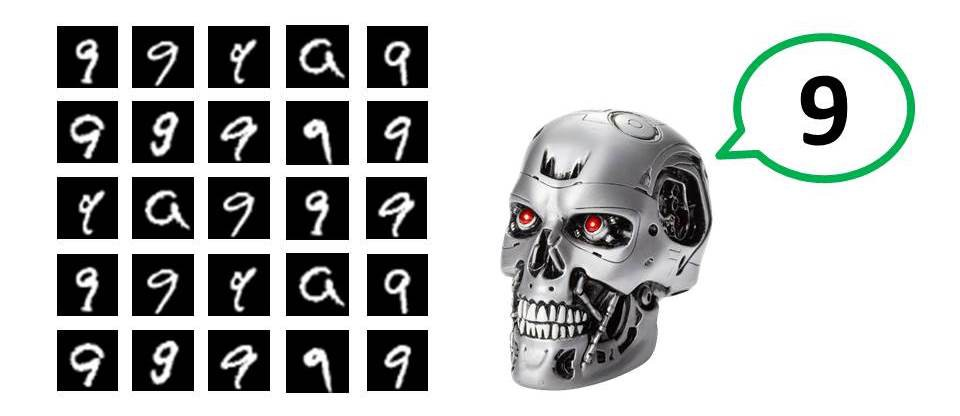
\includegraphics[width=1.1\textwidth,height=\textheight]{img/README/portada.jpeg}

\pagebreak
\end{frame}

\begin{frame}{Capítulo 0 Estructura del repositorio}
\protect\hypertarget{capuxedtulo-0-estructura-del-repositorio}{}
\begin{figure}
\centering
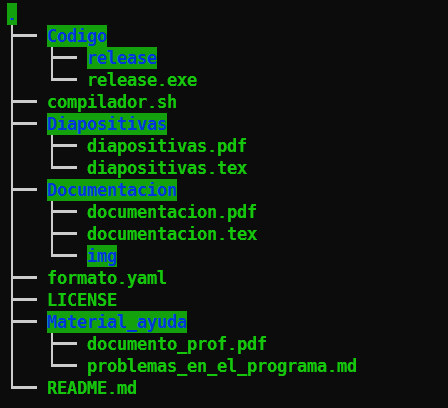
\includegraphics{img/README/Screenshot_1.png}
\caption{Tabla de contenido del repositorio}
\end{figure}
\end{frame}

\begin{frame}{Capítulo 1 Introducción}
\protect\hypertarget{capuxedtulo-1-introducciuxf3n}{}
La clasificación de imágenes es un concepto bastante viejo, aunque no
pareciese así, digamos que tiene entre 50 y 60 (1960-1970) años la
primera vez que se utilizó una tecnología así, sólo que esa vez era más
primitiva, por varias razones, tenemos que pensar que en ese tiempo las
computadoras, todavía trabajaban con grandes computadoras que ocupaban
un cuarto, todavía no estaba la teoría para la creación

Pero ¿Qué era lo que realmente realizaba? La clasificación entre hombres
y mujeres. ¿Cómo lo realizaba? Primero quiero que te imágenes señoritas
vestidas con pelo más abultado que el de los caballeros, sólo se usaba
foto de los hombros hacia arriba, se usaban sensores sensibles a la luz,
para poder pasar fotografías analógicas a digital, posterior a ello este
daba un mensaje diciendo si era hombre o mujer, es un excelente
antecedente de clasificación de imágenes.

Empezamos con el siguiente investigador que se acerca más a lo que es mi
proyecto, ya que el uso celdas foto sensibles para pasar trazos a
letras, esto es para digitalizarlos, pero además le enseño a hablar, es
decir pronunciar las palabras en el lenguaje inglés, resumiendo esto, el
hizo una clasificación de letras y además una red neural para que
pudieran hablar.

\begin{figure}
\centering
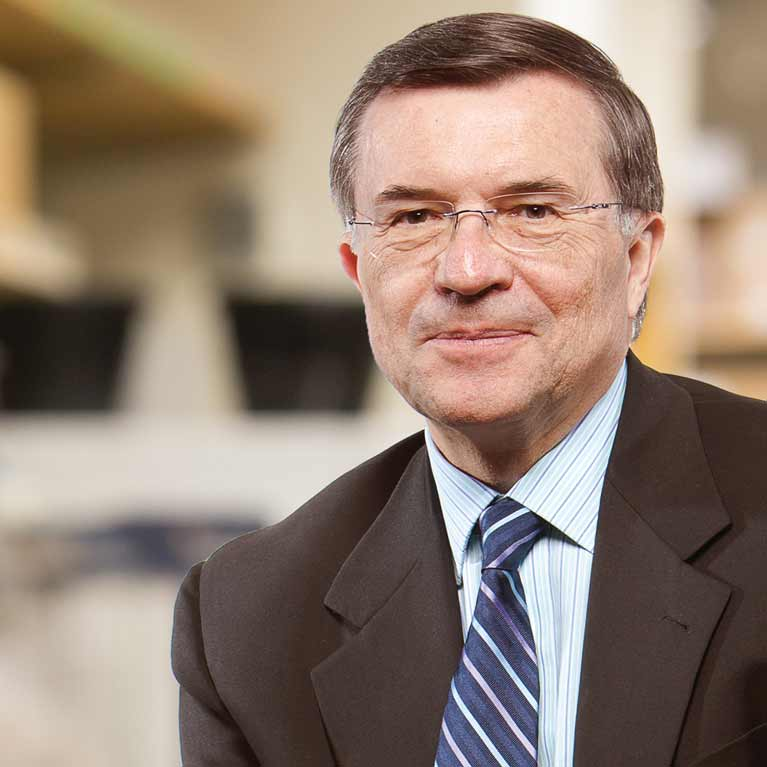
\includegraphics[width=0.3\textwidth,height=\textheight]{img/README/terrence.jpg}
\caption{Phd. Terrence Sejnowski}
\end{figure}

Retomando lo hecho por los antes mencionados, implementó, pero ahora
usando computadoras modernas, y con mucha mayor potencia, que aquellos
tiempos, y ahora todo siendo digital, mediante lenguajes de programación
y probabilidad, en lugar de redes neuronales como en 1986.
\end{frame}

\begin{frame}[fragile]{Definición del problema}
\protect\hypertarget{definiciuxf3n-del-problema}{}
En el proyecto anterior se tenía que utilizar el teorema de Bayes para
poder calcular la probabilidad y con dicho programa vamos a partir, es
decir que los conceptos asociados al calculo de probabilidades mediante
Bayes, ya se pueden calcular.

Definimos una imagen de \(X,Y\) dimensiones dadas en \texttt{pixeles},
cada pixel tiene 3 canales de color RGB con los cuales podemos
modificar. Cada imagen tendrá que ser clasificada dentro de una de las
posibles opciones de los datos entrenados, suponga que existen
\(C=[c_1,c_2,c_3, \cdots,c_n]\) clasificaciones con las que fue
entrenado, la imagen se pasará por el programa y dirá \(c_j\) es la
clasificación más probable o más parecida.

Vamos a definir la entrada, que en realidad son dos diferentes entradas,
por una parte tenemos al data-set para entrenar a nuestro modelo, piense
que tenemos una imagen de \(X,Y\) dimensiones y el otro imágenes que
tendremos que hacer pruebas, pero a diferencia de el set que esta
contenido en dimensiones especificas y con colores especificos, las
imagenes con las que se tienen que clasificar, no cuentan con dichas
características.

En este caso \(C=[0,1,2, \cdots,9]\)\hspace{0pt}. Nuestro objetivo es
detectar el número {[}0-9{]} por tanto, cada símbolo de este conjunto
tiene que tener un conjunto de imagenes que compartan una tendencia, por
ejemplo tener 100 imágenes de el número 1 desde diferentes posiciones y
rotaciones, con ello mediante expresiones matemáticas intentaremos
modelar un comportamiento que prediga el conjunto de datos abstrayendo
lo más importante.

En el caso de este proyecto se ha delimitado a que las imágenes de
entrenamiento tengan un dimensión de \(X,Y\) de \(32,32\) . Esto tiene
la razón de para limitar el tiempo de procesamiento de entrenamiento,
además de que el peso del repositorio no se eleve mucho. La
recomendación viene dada de un data-set real que tenia para
reconocimiento de letras que tenia un peso de \(1[Gb]\) y con ello
contaba con al rededor de \textbf{307,200} imagenes de entrenamiento.

Recordando que en este caso que dado un vector de condiciones
\(\vec{Q}\) que contiene los valores \([q_1,q_2,...,q_j]\) para \(j\)
condiciones, a los cuales debe igualarse \(Am_i\), obtener
\(Y_{max}(\vec{Q})\) que es la probabilidad más grande para dicho
vector.

Para solucionar el problema tenemos que calcular la probabilidad pixel y
pixel \[
P(Y=y_i|X=x_o)= \frac{P(X=x_0| Y=y_i)\cdot P(Y=y_i)}{P(X=x_o)}
\]
\end{frame}

\begin{frame}[fragile]{Solución}
\protect\hypertarget{soluciuxf3n}{}
\begin{block}{Teoría}
\protect\hypertarget{teoruxeda}{}
\begin{block}{Primer paso , elaboración de data-set}
\protect\hypertarget{primer-paso-elaboraciuxf3n-de-data-set}{}
En este caso son 10 conjuntos de imágenes, cada uno con 15 imágenes como
se aprecia en este caso para \(C_1=1\)

\begin{figure}
\centering
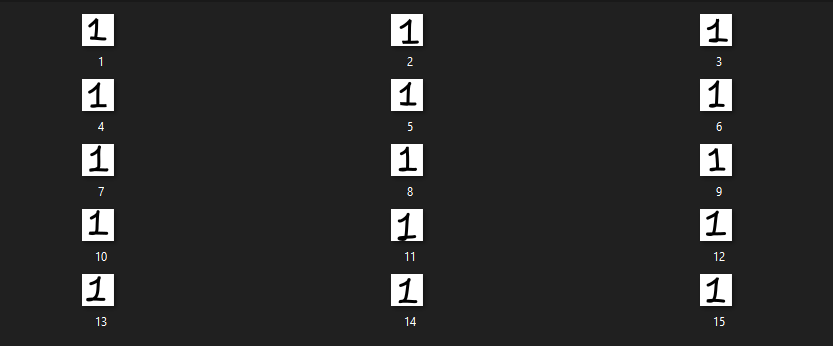
\includegraphics{img/README/image-20220506183750690.png}
\caption{data-set número 1}
\end{figure}
\end{block}

\begin{block}{Segundo paso, elaboración de historiagrama}
\protect\hypertarget{segundo-paso-elaboraciuxf3n-de-historiagrama}{}
Para este método de predicción tenemos que que tomar
\(32 \hspace{0.3cm}x \hspace{0.3cm} 32=1024\) .Será un histograma que
contiene el número que que tan negro es, si este es 0 significa que lo
es, sin embargo si es 255 es blanco, si es un intermedio entre estos es
un gris. Sólo tenemos esos dos, ya que limitamos nuestra entrada a
dichos dos colores, para simplificar, si una entrada fuera de otro color
tendríamos que cambiarla a grises, ya que los que nos interesa en esta
clasificación es la forma, no el color.

primero definamos los valores de las imágenes para un modelo, suponga la
existencia de un conjunto de imagenes de comparten las siguientes
características \textbf{\{escala de grises, están escritos a mano,
tienen la mismas dimensiones, esta escrito el mismo número\}}.

Veamos un ejemplo para las características anteriormente dadas para el
modelo del número \texttt{1} definamos las características:

\{escala de gristes,escritos a mano,tienen dimensión 32x32,el número es
1 y son 15 elementos imagenes\}

Con el anterior conjunto podemos obtener que \(n=15\) \(x=32,y=32\)

Definamos que una imagen es lo siguiente \[
I=
\begin{pmatrix}
p[0,0] & p[0,1] & \cdots & p[0,x]\\
p[1,0] & p[1,1] & \cdots & p[1,x]\\
\vdots & \vdots & \ddots & \vdots\\
p[y,0] & p[y,0] & \cdots & p[y,x]
\end{pmatrix}
\] Como vamos a trabajar con varias imágenes es necesario definir una
pequeña notacion \(p1[0,0]\) este es el pixel {[}0,0{]} para la
\textbf{imagen 1}, \(pn[0,0]\) es el pixel {[}0,0{]} de la
\texttt{n-esima} imágen.

También definiré una matriz llama \(M=media\) , en este caso tiene un
subíndice \(1\) eso significa que es la matriz media de imagenes 1 \[
M_1=
\begin{pmatrix}
pm[0,0] & pm[0,1] & \cdots & pm[0,x]\\
pm[1,0] & pm[1,1] & \cdots & pm[1,x]\\
\vdots & \vdots & \ddots & \vdots\\
pm[y,0] & pm[y,0] & \cdots & pm[y,x]
\end{pmatrix}
\] para calcular cada uno de los puntos de la matriz \(M\) usamos lo
siguiente \[
pm[0,0]= \frac{p1[0,0]+ p2[0,0] + p3[0,0]+ \cdots + pn[0,0]}{n}
\] Es la media aritmética para el pixel 1 de las imágenes de número 1,
se tiene que realizar lo mismo para todos los los pixeles de la matriz
\(M\), pero terminar todos los puntos de la matriz \(M\) sería el modelo
sólo para la imágenes con el número 1 pero para ser un clasificador
tiene que tener más que de sólo un sólo resultado, y para este proyecto
tiene que clasificar entre los posibles resultados de
\([0,1,2,3,4,\cdots,9]\) y por tanto tendríamos los modelos
\([M_0,M_1,M_2,M_3,M_4,\cdots,M_9]\).
\end{block}

\begin{block}{Tercer paso tratar la imagen}
\protect\hypertarget{tercer-paso-tratar-la-imagen}{}
La entrada no es siempre la que queremos y por ello es necesario
manipularla de tal manera que la entrada coincida con una entrada que
sea posible tratarla.

Para resolver el problema, vamos a usar el teorema de Bayes con la
siguiente ecuación: \[
P(Y=y_i|X=x_o)= \frac{P(X=x_0| Y=y_i)\cdot P(Y=y_i)}{P(X=x_o)}
\] Con dicha ecuación empleándola sobre una imagen podemos saber cuando
es la probabilidad por cada pixel de la imagen que queremos clasificar
\[
P(Y=y_i) \hspace{1cm} \text{Probabilidad a priori}
\]

\[
P(X=x_0| Y=y_i) \hspace{1cm} \text{Probabilidad a posterior}
\]

\[
P(X=x_o) \hspace{1cm} \text{Termino de normalización}
\]

\[
P(Y=y_i|X=x_o)  \hspace{1cm} \text{Probabilidad  de que un pixel sea un modelo}
\]

Vamos desglosando cada uno en el orden anterior

\begin{block}{Probabilidad a priori}
\protect\hypertarget{probabilidad-a-priori}{}
Definamos las variables \(yi \in \{0,1,2,\cdots,9\}\) ya que son las
posibles categorías que hay , es decir que es la \textbf{probabilidad de
que sea alguna de las categorías} y por tanto se calcula de la siguiente
manera \[
P(Y=y_i)=\frac{1}{n}=\frac{1}{10}\%
\] recuerda que \(n\) es el número de modelos.

Hay que tener en consideración que esto es debido a que todos los
modelos se entrenaron con el mismo número de imágenes, de no ser así la
formula sería : \[
P(Y=y_i)=\frac{\text{Num imagenes modelo }y_i}{\text{Num imagenes totales}}
\] Si para entrenar cada modelo usaste 15 imágenes y son 10 modelos
entonces tendrías \$150 \$ imagenes totales.

Como para el modelo \texttt{Num\ imagenes\ modelo} \(y_i\) fueron 15
imágenes para entrenar a este modelo, por tanto \[
\text{Num imagenes modelo }y_i=15
\] Entonces la probabilidad para que el modelo sea igual a 1 \(P(Y=1)\)
: \[
P(Y=1)=\frac{15}{150}\%
\]
\end{block}

\begin{block}{Probabilidad a posterior}
\protect\hypertarget{probabilidad-a-posterior}{}
Es una probabilidad condicional y por ello recordar la fórmula \[
P(B|A)=\frac{P(A\cap B)}{P(A)}
\] Entonces utilizamos la anterior formula \[
P(X=x_0| Y=y_i)=\frac{P(X=x_o\cap Y=y_i)}{P(X=x_o)}
\] Esta probabilidad te dice \textbf{que tan probable es que dado un
modelo, el pixel } \(X=x_o\) sea del valor esperado. \[
P(X=x_o)
\]

Te dice de \textbf{cual es la probabilidad de que el pixel tenga el
valor dado}, por ejemplo
\end{block}
\end{block}

\begin{block}{Cuarto paso obtener la probabilidad de una imagen}
\protect\hypertarget{cuarto-paso-obtener-la-probabilidad-de-una-imagen}{}
Para la solución requerimos saber de dos cosas:

\begin{itemize}
\tightlist
\item
  Teorema de Bayes para implementar la probabilidad.
\item
  Una imagen que no pertenezca al data-set con el cual entrenamos los
  modelos.
\end{itemize}

Pasamos la imagen \textbf{input} que queremos saber a que clasificación
pertenece, llamaremos a la matriz \(I\).

Siguiendo los siguientes pasos:

\begin{itemize}
\tightlist
\item
  Calcular la probabilidad a priori es a partir del número de modelos.
\item
  Tratar la imagen y darle las dimensiones, y subir los colores negros
  para que sean más negros y los blancos , sean más blancos, es decir
  que si es cercano a blanco volverlo totalmente blanco y si es cercano
  a negro volverlo totalmente negro.
\item
  Calcular la probabilidad a posteriori, pixel a pixel.
\item
  Seleccionar la imagen con mayor coincidencia.
\end{itemize}

\begin{block}{Quinto paso obtener tiempo de ejecución y precisión}
\protect\hypertarget{quinto-paso-obtener-tiempo-de-ejecuciuxf3n-y-precisiuxf3n}{}
\begin{block}{Tiempo de ejecución}
\protect\hypertarget{tiempo-de-ejecuciuxf3n}{}
Para lograr dicho objetivo sólo es necesario que se pueda calcular el
tiempo en que tarda desde que la imagen es leida, posteriormente tratada
y obtenido su probabilidad, con ello podemos decir que se obtiene el
tiempo.
\end{block}

\begin{block}{Precisión}
\protect\hypertarget{precisiuxf3n}{}
En el caso de la precisión, tenemos que tomar 3 casos de dificultad y
para lograr ello vamos a hacer algo muy simple, la regla del 80\% de
casos para entrenar y el 20\% para probar el resultado, en este caso, el
conjunto de datos de entrenamiento que tenemos es limitado y por ello
tenemos que reducir la prueba a los siguientes

\begin{itemize}
\tightlist
\item
  Fácil: entrenar el modelo con 4 imágenes por cada modelo y comprobar
  el resultado con una.
\item
  Medio: entrenar el modelo con 5 imágenes por cada modelo y comprobar
  el resultado con 2.
\item
  Difícil: entrenar el modelo con 7 imágenes por cada modelo y comprobar
  el resultado con 3.
\item
  imposible: entrenar el modelo con 10 imágenes por cada modelo y
  comprobar el resultado con 4.
\end{itemize}
\end{block}
\end{block}
\end{block}
\end{block}

\begin{block}{Pseudocódigo}
\protect\hypertarget{pseudocuxf3digo}{}
\begin{Shaded}
\begin{Highlighting}[]
\NormalTok{Menu()}
    \ControlFlowTok{if} \DecValTok{1}\NormalTok{ then:}
\NormalTok{        generarModelos()}
    \ControlFlowTok{elif} \DecValTok{2}\NormalTok{:}
\NormalTok{        cargarModelosAMemoria()}
    \ControlFlowTok{elif} \DecValTok{3}\NormalTok{:}
\NormalTok{        cargarImagenAmemoria()}
\NormalTok{        tratarImagen()}
\NormalTok{        calcularProbabilidadImagen()}
\NormalTok{        seleccionarModeloMasParecido()}
   \ControlFlowTok{elif} \DecValTok{4}\NormalTok{:}
\NormalTok{        EjecutarTestPrecision()}
\end{Highlighting}
\end{Shaded}
\end{block}
\end{frame}

\begin{frame}[fragile]{Experimentos}
\protect\hypertarget{experimentos}{}
\begin{block}{Baja dificultad ( 3 casos )}
\protect\hypertarget{baja-dificultad-3-casos}{}
Son 3 imagen con resolución 32x32=1024 puntos (1x el pincel)

\begin{block}{Problema 1}
\protect\hypertarget{problema-1}{}
\begin{figure}
\centering

\includegraphics[width=0.72917in,height=\textheight]{img/README/1-16526373701691.png}
\caption{1}
\end{figure}

\begin{verbatim}
Tu imagen es: ..\entrenado\1.jpg
La probabilidad es: 0.06260569852941193
La probabilidad de coincidencia es :0.6260569852941194
El tiempo fue:0.171875 segundos
\end{verbatim}

\begin{itemize}
\tightlist
\item
  La predicción es correcta
\end{itemize}
\end{block}

\begin{block}{Problema 2}
\protect\hypertarget{problema-2}{}
\begin{figure}
\centering

\includegraphics[width=0.72917in,height=\textheight]{documentacion/img/2.png}
\caption{Imagen 2}
\end{figure}

\begin{verbatim}
Tu imagen es: ..\entrenado\3.jpg
La probabilidad es: 0.0598081341911768
La probabilidad de coincidencia es :0.598081341911768
El tiempo fue:0.171875 segundos
\end{verbatim}

\begin{itemize}
\tightlist
\item
  La predicción es incorrecta.
\end{itemize}
\end{block}

\begin{block}{Problema 3}
\protect\hypertarget{problema-3}{}
\begin{figure}
\centering

\includegraphics[width=0.72917in,height=\textheight]{documentacion/img/3.png}
\caption{Imagen 3}
\end{figure}

\begin{verbatim}
Tu imagen es: ..\entrenado\3.jpg
La probabilidad es: 0.06111825980392147
La probabilidad de coincidencia es :0.6111825980392147
El tiempo fue:0.171875 segundos
\end{verbatim}

\begin{itemize}
\tightlist
\item
  La predicción es correcta
\end{itemize}
\end{block}
\end{block}

\begin{block}{Media dificultad ( 3 casos )}
\protect\hypertarget{media-dificultad-3-casos}{}
Son 3 imagenes con resolución 144x144, es un 20x (x3 el pincel) a baja
dificultad.

\begin{block}{Problema 1}
\protect\hypertarget{problema-1-1}{}
\begin{figure}
\centering

\includegraphics[width=0.72917in,height=\textheight]{documentacion/img/4.png}
\caption{Imagen 4}
\end{figure}

\begin{verbatim}
Tu imagen es: ..\entrenado\4.jpg
La probabilidad es: 0.06125340413942622
La probabilidad de coincidencia es :0.6125340413942622
El tiempo fue:3.234375 segundos
\end{verbatim}

\begin{itemize}
\tightlist
\item
  La predicción es correcta.
\end{itemize}
\end{block}

\begin{block}{Problema 2}
\protect\hypertarget{problema-2-1}{}
\begin{figure}
\centering
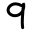
\includegraphics[width=0.72917in,height=\textheight]{documentacion/img/5.png}
\caption{Imagen 5}
\end{figure}

\begin{verbatim}
Tu imagen es: ..\entrenado\5.jpg
La probabilidad es: 0.06304971178286195
La probabilidad de coincidencia es :0.6304971178286195
El tiempo fue:1.671875 segundos
\end{verbatim}

\begin{itemize}
\tightlist
\item
  La predicción es correcta.
\end{itemize}
\end{block}

\begin{block}{Problema 3}
\protect\hypertarget{problema-3-1}{}
\begin{figure}
\centering

\includegraphics[width=0.72917in,height=\textheight]{documentacion/img/6.png}
\caption{Imagen 6}
\end{figure}

\begin{verbatim}
Tu imagen es: ..\entrenado\6.jpg
La probabilidad es: 0.06176663489469558
La probabilidad de coincidencia es :0.6176663489469558
El tiempo fue:1.75 segundos
\end{verbatim}
\end{block}
\end{block}

\begin{block}{Alta dificultad ( 3 casos )}
\protect\hypertarget{alta-dificultad-3-casos}{}
Son 3 imagenes con resolución de 320x320 =102,400 por tanto es un
multiplicador de 100x (x10 el pincel).

\begin{block}{Problema 1}
\protect\hypertarget{problema-1-2}{}
\begin{figure}
\centering

\includegraphics[width=0.72917in,height=\textheight]{documentacion/img/7.png}
\caption{Imagen 7}
\end{figure}

\begin{verbatim}
Tu imagen es: ..\entrenado\7.jpg
La probabilidad es: 0.0632344898896487
La probabilidad de coincidencia es :0.632344898896487
El tiempo fue:7.4375 segundos
\end{verbatim}

\begin{itemize}
\tightlist
\item
  La predicción es correcta.
\end{itemize}
\end{block}

\begin{block}{Problema 2}
\protect\hypertarget{problema-2-2}{}
\begin{figure}
\centering

\includegraphics[width=0.72917in,height=\textheight]{documentacion/img/8.png}
\caption{Imagen 8}
\end{figure}

\begin{verbatim}
Tu imagen es: ..\entrenado\8.jpg
La probabilidad es: 0.06314603247545689
La probabilidad de coincidencia es :0.6314603247545688
El tiempo fue:7.125 segundos
\end{verbatim}

\begin{itemize}
\tightlist
\item
  La predicción es correcta.
\end{itemize}
\end{block}

\begin{block}{Problema 3}
\protect\hypertarget{problema-3-2}{}
\begin{figure}
\centering

\includegraphics[width=0.72917in,height=\textheight]{documentacion/img/9.png}
\caption{Imagen 9}
\end{figure}

\begin{verbatim}
Tu imagen es: ..\entrenado\9.jpg
La probabilidad es: 0.06002850413596944
La probabilidad de coincidencia es :0.6002850413596944
El tiempo fue:7.296875 segundos
\end{verbatim}

\begin{itemize}
\tightlist
\item
  La predicción es correcta.
\end{itemize}
\end{block}
\end{block}

\begin{block}{Sin solución (1 caso)}
\protect\hypertarget{sin-soluciuxf3n-1-caso}{}
Una imagen con una resolución de 1024x1024= 1,048,576 por tanto es un
multiplicador de 1024x (x32 el pincel).

\begin{figure}
\centering

\includegraphics[width=0.72917in,height=\textheight]{documentacion/img/0.png}
\caption{Imagen 10}
\end{figure}

\begin{verbatim}
Tu imagen es: ..\entrenado\5.jpg
La probabilidad es: 0.05316162071969969
La probabilidad de coincidencia es :0.5316162071969969
El tiempo fue:70.53125 segundos
\end{verbatim}

\begin{itemize}
\tightlist
\item
  La predicción es incorrecta.
\item
  Este decimos que es el caso imposible porque de aquí hacia arriba es
  el punto sin retorno, es posible que se ejecute o que no, todo es
  culpa de las limitaciones por default de Python, el programa esta
  hecho para soportar cualquier tamaño de imagen, es decir que si se
  incluye una imagen que de \(4096x4096\) es decir multiplicar por 4 la
  anchura y la altura, aproximadamente tardaría \(32\) minutos en
  procesarse, si de multiplicara x2 la anchura y la altura,
  automáticamente tardaría 2 horas, por ello puedes probar con una
  imagen de \(8192x8192\).
\end{itemize}

\begin{verbatim}
RuntimeWarning: overflow encountered in ubyte_scalars
  resta.append(abs(modelo[i]-imagen[i]))
\end{verbatim}
\end{block}

\begin{block}{Resultados test precisión}
\protect\hypertarget{resultados-test-precisiuxf3n}{}
\begin{verbatim}
 product: AMD Ryzen 7 2700 Eight-Core Processor
          vendor: Advanced Micro Devices [AMD]
          8 nucleos 16 hilos
- 128 gb DDR4 2600mhz
- Windows 10 pro
\end{verbatim}

\begin{longtable}[]{@{}llll@{}}
\toprule
Dificultad & Datos entrenamiento & Datos test & Precisión
\%\tabularnewline
\midrule
\endhead
Baja & 4 & 1 & 70\tabularnewline
Media & 5 & 2 & 90\tabularnewline
Alta & 7 & 3 & 96.666\tabularnewline
Imposible & 10 & 4 & 95\tabularnewline
\bottomrule
\end{longtable}

La ejecución de resultados es :

\begin{verbatim}
[70.0, 90.0, 96.66666666666667, 95.0]
El tiempo fue:18.296875 segundos
\end{verbatim}
\end{block}

\begin{block}{Resultados tiempo de ejecución}
\protect\hypertarget{resultados-tiempo-de-ejecuciuxf3n}{}
Para las pruebas se uso el siguiente hardware:

\begin{verbatim}
 product: AMD Ryzen 7 2700 Eight-Core Processor
          vendor: Advanced Micro Devices [AMD]
          8 nucleos 16 hilos
- 32 gb DDR4 2600mhz
- Windows 10 pro
\end{verbatim}

\begin{longtable}[]{@{}lll@{}}
\toprule
Dificultad & Tiempo {[}s{]} & Multiplicador\tabularnewline
\midrule
\endhead
Baja & 0.171875 & x1\tabularnewline
Media & 3.234375 & x4\tabularnewline
Alta & 7.125 & x100\tabularnewline
Imposible & 70.53125 & x1024\tabularnewline
\bottomrule
\end{longtable}

La variable en el eje X=multiplicador, en el eje Y=tiempo

\begin{figure}
\centering
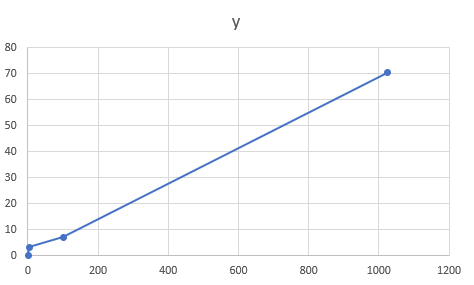
\includegraphics{img/README/image-20220516004324192.png}
\caption{Grafica dependiente del multplicador}
\end{figure}

Con la gráfica obtenemos que el crecimiento de tiempo es lineal.
\end{block}
\end{frame}

\begin{frame}{Capítulo 3 Conclusión}
\protect\hypertarget{capuxedtulo-3-conclusiuxf3n}{}
\begin{block}{Barrera Peña Víctor Miguel}
\protect\hypertarget{barrera-peuxf1a-vuxedctor-miguel}{}
El proyecto se terminó cumpliendo todos los objetivos que planteaba el
proyecto, se pudo lograr un clasificador muy versátil que puede
entrenarse para clasificar cualquier clase de letras escritas a mano o
incluso para reconocer caracteres de texto, por ejemplo de latex, lo
único que tendría que hacerse es crear los data-set para el fin que se
busca y con ello se lograría el objetivo concluido, por tanto puedo
decir que es un excelente programa. Esta relizado de manera que se puede
extender para reconocer más caracteres, tiene un precisión alta, puede
entrenarse con facilidad, puede detectar imagenes de diferentes tamños,
creo que el programa supera las espectativas con las que fue diseñado,
no hay algo que pueda mejorar en este momento y por ello creo que el
proyecto es excelente.
\end{block}

\begin{block}{Espino de Horta Joaquín Gustavo}
\protect\hypertarget{espino-de-horta-joaquuxedn-gustavo}{}
La implementación de esta nueva característica o al menos un nuevo
enfoque al algoritmo del teorema de Bayes se realizó adantándose al
problema que ya se tenía presente, conservando el principio operativo,
aplicado a una comparativa de una sola dimensión para daterminar el
reconocimiento de patrones, podrían hacerse sencillas modificaciones
como el reconocimiento de color, distancia o siluetas así como
algoritmos de recorte de imagen.

Obteniendo un resultado de calidad comercial al reconocimiento de
objetos ubicando en una gran imagen proveniente de una transmisión en
video a identificar en tiempo real. Como lo son los códigos QR, letras,
números, incluso rostros o retinas entre otros dispositivos.

También pueden aplicarse a la edición de imágenes, aplicando selecciones
inteligentes, reconociendo patrones y convirtiendo dibujos en mapas de
vectores de manera automática. Incluso implementarlos en la generación
procedural de la música tonal.
\end{block}
\end{frame}

\begin{frame}{Anexo}
\protect\hypertarget{anexo}{}
\begin{block}{Elaboración de data-set}
\protect\hypertarget{elaboraciuxf3n-de-data-set}{}
Para crear los data-set se uso el programa de Inkscape con siguientes
requisitos:

\begin{itemize}
\tightlist
\item
  imágenes cuadradas
\item
  Usando la plumilla en color negro de acuerdo al multiplicador de cada
  tipo de imagen, por ejemplo la imagen de \(32x32\) tiene un
  multiplicador de \(1\) por tanto la plumilla tiene que tener un tamaño
  de \(1.0[mm]\), si la imagen fuera de \(144x144\) el multiplicador es
  \(x3\), ya que \(\frac{144}{33} \approx 3\).
\end{itemize}

Como seleccionar tamaño plumilla:

\begin{figure}
\centering
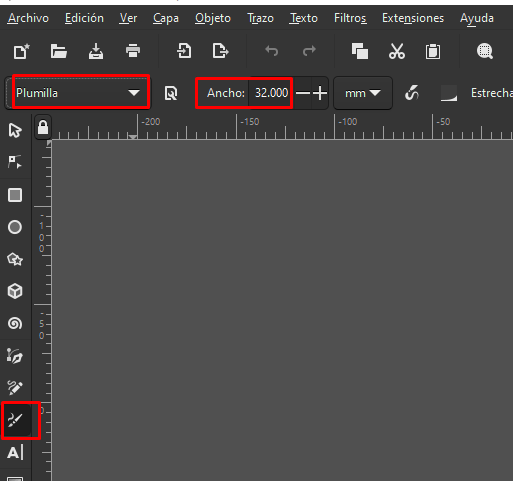
\includegraphics{img/README/image-20220516010023659.png}
\caption{seleccionar tamaño plumilla}
\end{figure}

Como seleccionar tamaño de imagen:

\begin{enumerate}
\tightlist
\item
  Ir a propiedades de documento
\end{enumerate}

\begin{figure}
\centering
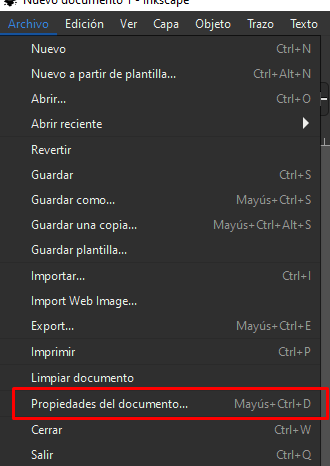
\includegraphics{img/README/image-20220516010118895.png}
\caption{image-20220516010118895}
\end{figure}

2.Cambiar dimensiones

\begin{figure}
\centering
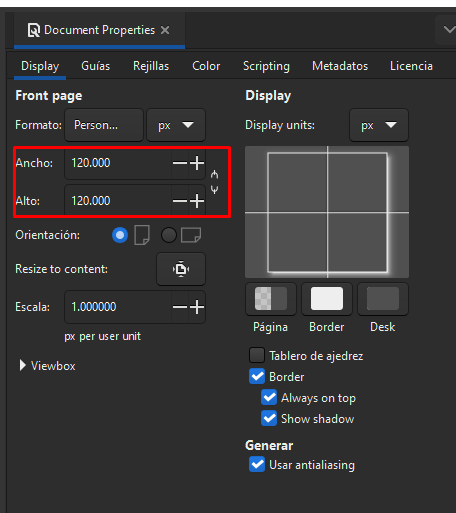
\includegraphics{img/README/image-20220516010209321.png}
\caption{cambiar dimensiones lienzo}
\end{figure}
\end{block}
\end{frame}

\begin{frame}{Referencias}
\protect\hypertarget{referencias}{}
\begin{itemize}
\tightlist
\item
  \emph{The evolution of image classification explained}. (z.d.). Image
  Classification. Geraadpleegd op 6 mei 2022, van
  https://stanford.edu/\%7Eshervine/blog/evolution-image-classification-explained
\item
  G. (2021, 14 mei). \emph{A brief history of Facial Recognition}. NEC.
  Geraadpleegd op 6 mei 2022, van
  https://www.nec.co.nz/market-leadership/publications-media/a-brief-history-of-facial-recognition/\#:\%7E:text=The\%20earliest\%20pioneers\%20of\%20facial,to\%20recognise\%20the\%20human\%20face.
\item
  \emph{History of Artificial Intelligence in hindi \textbar{} Brief
  history \textbar{} MCA/B.tech,etc \textbar{} ai history}. (2021, 4
  oktober). YouTube. Geraadpleegd op 6 mei 2022, van
  https://www.youtube.com/watch?v=3qRJfUv7W\_Y
\item
  \emph{1 - Bayes con imágenes - Introducción}. (2020, 7 april).
  YouTube. Geraadpleegd op 15 mei 2022, van
  https://www.youtube.com/watch?v=qI3n3x4DldY
\item
  -\emph{2 - Bayes con imágenes - modelo 1}. (2020, 7 april). YouTube.
  Geraadpleegd op 15 mei 2022, van
  https://www.youtube.com/watch?v=bCVQIfm4YFI
\item
  \emph{3 - Bayes con imágenes - modelo 2}. (2020, 7 april). YouTube.
  Geraadpleegd op 15 mei 2022, van
  https://www.youtube.com/watch?v=zarhUCRGR14
\item
  \emph{4 - Bayes con imágenes - modelo 3}. (2020, 7 april). YouTube.
  Geraadpleegd op 15 mei 2022, van
  https://www.youtube.com/watch?v=q9juEGJb3mM
\item
  \emph{5 - Bayes con imágenes - modelo 4}. (2020, 7 april). YouTube.
  Geraadpleegd op 15 mei 2022, van
  https://www.youtube.com/watch?v=ez8aht07Rqk
\item
  \emph{6 - Bayes con imágenes - Conclusiones}. (2020, 7 april).
  YouTube. Geraadpleegd op 15 mei 2022, van
  https://www.youtube.com/watch?v=9HOrMUNw\_pA
\end{itemize}
\end{frame}

\end{document}
